
\chapter{Funciones reales de variable real}

\PartialToc

\hypersetup{linkcolor=ptctitle}

\vspace*{0.5cm}
 
\begin{flushright}
\textit{\footnotesize{}El matemático P.G Lejeune Dirichlet }
\par\end{flushright}{\footnotesize \par}

\begin{flushright}
\textit{\footnotesize{}no era muy amigo de escribir cartas.}
\par\end{flushright}{\footnotesize \par}

\begin{flushright}
\textit{\footnotesize{}Hizo una excepción cuando nació }
\par\end{flushright}{\footnotesize \par}

\begin{flushright}
\textit{\footnotesize{}su primer hijo. Dirichlet mando un }
\par\end{flushright}{\footnotesize \par}

\begin{flushright}
\textit{\footnotesize{}telegrama a su suegro con siguiente }
\par\end{flushright}{\footnotesize \par}

\begin{flushright}
\textit{\footnotesize{}mensaje << 2+1=3>>. }
\par\end{flushright}{\footnotesize \par}

\begin{flushright}
{\small{} }\textbf{\textit{Dirichlet}}: 
\par\end{flushright}

\vspace*{-1mm}


\section{Funciones reales de variable real.}

Las funciones son las herramientas principales para la descripción
matemática de una situación real. Todas las \emph{fórmulas} de la
Física no son más que funciones: expresan cómo ciertas magnitudes
(por ejemplo el volumen de un gas) dependen de otras (la temperatura
y la presión). El concepto de función es tan importante que muchas
ramas de la matemática moderna se caracterizan por el tipo de funciones
que estudian. No es de extrañar, por ello, que el concepto de función
sea de una gran generalidad. Además, se trata de uno de esos conceptos
cuyo contenido esencial es fácil de comprender pero difícil de formalizar.

\begin{defi}{Función}{} Sean $A$ y $B$ dos conjuntos. Una función
de $A$ en $B$ es una \emph{regla} que \emph{a cada elemento de $A$
asocia un único elemento de $B$.} \end{defi}

En esta definición la dificultad radica en precisar matemáticamente
lo que se entiende por \emph{regla}. Como solamente vamos a trabajar
con funciones elementales considero que no es necesario dar más precisiones.

Observa que una función son \emph{tres} cosas: el conjunto $A$ donde
está definida, el conjunto $B$ donde toma valores y la regla que
la define. En este curso estamos interesados principalmente en funciones
entre conjuntos de números reales, es decir, $A$ y $B$ son subconjuntos
de \R; con frecuencia $B=\R$. Estas funciones se llaman \emph{funciones
reales de una variable real}.

\noindent {\textbf{Convenio.}}\ En lo que sigue solamente consideraremos
funciones reales y, si no se especifica otra cosa, se entiende que
$B=\R$.

Por tanto, para darnos una función nos deben decir, en principio,
el subconjunto $A$ de \R\ donde suponemos que la función está definida
y la regla que asigna a cada número de $A$ un único número real.
El conjunto $A$ recibe el nombre de \emph{dominio} de la función.

Las funciones se representan por letras. En la práctica las letras
más usadas son $f$, $g$ y $h$, pero cualquiera otra es también
buena. Si $f$ es una función y $x$ es un número que está en su dominio,
se representa por $f(x)$ (léase ``$f$ de $x$'' o, mucho mejor,
``$f$ evaluada en $x$'' o ``el valor de $f$ en $x$'') el número
que $f$ asigna a $x$, que se llama \emph{imagen de $x$ por $f$
}.

\emph{Es muy importante distinguir entre $f$ (una función) y $f(x)$
(un número real)}.

El símbolo \funcreal{f}{A}\ se utiliza para indicar que $f$
es una función \emph{cuyo dominio es} $A$ (se supone, como hemos
dicho antes, que $A$ es un subconjunto de \R). También es frecuente
usar el simbolismo $\,x\mapsto f(x)$, $(x\in A)$.

Es importante advertir\marginpar{\flushright\curvasr} que las propiedades
de una función dependen de la regla que la define \emph{y también
de su dominio}, por ello \emph{dos funciones que tienen distintos
dominios se consideran distintas funciones aunque la regla que las
defina sea la misma.} 

\begin{defi}{Igualdad de funciones}{} Dos funciones $f$ y $g$ son
iguales cuando tienen igual dominio y $f(x)=g(x)$ para todo $x$
en el dominio común. \end{defi}

Notemos también que aunque estamos acostumbrados a representar a las
funciones mediante \emph{fórmulas}, no siempre es posible hacerlo.
\begin{ejemplo} Consideremos las funciones siguientes. \begin{enumerate}

\item \ \funcreal{f}{\R}\ la función dada por $f(x)=x^{2}$. 

\item \ \funcreal{g}{\Rp}\ la función dada por $g(x)=x^{2}$. 

\item \ \funcreal{h}{\R}\ la función dada por\ $h(x)=\begin{cases}
1,\  & \text{si \ensuremath{x\in\Q}}\\
-1,\  & \text{si \ensuremath{x\in\R\setminus\Q}}
\end{cases}$ 

\item \ Sea $\,f(x)=\dis\frac{x^{3}+5x+6}{x^{2}-1}$

\end{enumerate} Según lo antes dicho, las funciones en a) y b) son
distintas. De hecho tienen propiedades distintas. Observa que la función
definida en b) es creciente y la definida en a) no lo es.\par La
función definida en c) es llamada \emph{función de Dirichlet}. Nótese
que no es fácil calcular los valores de dicha función porque no siempre
se sabe si un número real dado es racional o irracional. ¿Es $\e+\pi$
racional? Pese a ello la función está correctamente definida.\par En
d) no nos dan explícitamente el dominio de $f$ por lo que se entiende
que $f$ está definida siempre que $f(x)$ tenga sentido, es decir,
siempre que, $x^{2}-1\neq0$, esto es, para $x\neq\pm1$. \end{ejemplo}

\noindent \textbf{El convenio del dominio.}\ Cuando una función se
define por una fórmula ``$f(x)\,$=\,fórmula'' y el dominio no
es explícito, se entiende que el dominio es el mayor conjunto de valores
de $x$ para los cuales la expresión $f(x)$ tiene sentido como número
real. Éste es el llamado \emph{dominio natural} de la función.

Dada una función \funcreal{f}{A}, y un conjunto no vacía $C\subset A$,
el conjunto de las imágenes por $f$ de todos los elementos de $C$:
\[
f(C)=\set{f(x):x\in C}
\]
se llama \emph{imagen de $C$ por $f$}. Cuando $C=A$, el conjunto
$f(A)$ se llama \emph{conjunto imagen} de $f$ y también \emph{rango}
o \emph{recorrido} de $f$. 

\subsection{Operaciones con funciones}

La mayoría de las funciones que vamos a usar en este curso pertenecen
a la clase de las \emph{funciones elementales}. Se llaman así porque
pueden obtenerse a partir de ciertos tipos de funciones bien conocidas
realizando las operaciones de suma, producto, cociente y composición
de funciones.

\noindent {\textbf{Suma, producto y cociente de funciones.}}\ Dadas
dos funciones \funcreal{f,g}{A}, se define su \emph{función suma}
(resp. \emph{producto}) como la función que a cada número $x\in A$
asigna el número real $f(x)+g(x)$ (resp. $f(x)g(x)$). Dicha función
se representa con el símbolo $f+g$ (resp. $fg$). Se define la función
cociente de $f$ por $g$ como la función que a cada número %
\mbox{%
$x\in A$ con $g(x)\neq0$%
} asigna el número real $\dis\frac{f(x)}{g(x)}$. Dicha función se
representa por $\dis\frac{f}{g}$. También podemos multiplicar una
función $f$ por un número $\alpha$ para obtener la función $\alpha f$
que asigna a cada $x\in A$ el número $\alpha f(x)$. De todas formas,
el producto de un número por una función puede considerarse como un
caso particular del producto de funciones, pues se identifica el número
$\alpha$ con la \emph{función constante} que toma como único valor
$\alpha$.

Las propiedades de la suma y el producto de funciones son las que
cabe esperar y su demostración es inmediata pues se reducen a las
correspondientes propiedades de los números. \begin{proposicion}{}{}
Cualesquiera sean las funciones \funcreal{f,g,h}{A}\ se verifican
las siguientes propiedades:\par Asociativas. \ $(f+g)+h=f+(g+h)$;\quad{}$(fg)h=f(gh)$\par Conmutativas.\ $f+g=g+f$;\quad{}$fg=gf$\par Distributiva.\ $(f+g)h=fh+gh$
\end{proposicion}

\begin{defi}\textbf{{Composición de funciones}{}}\ Sean \funcreal{f}{A}\ y
\funcreal{g}{B}\ funciones con %
\mbox{%
$f(A)\subset B$%
}. En tal caso, la función \funcreal{h}{A}\ dada por $h(x)=g(f(x))$
para todo $x\in A$ se llama \emph{composición de $g$ con $f$} y
se representa por $h=g\circ f$. Observa que la función $g\circ f$,
solamente está definida cuando la imagen de $f$ está contenida en
el dominio de $g$. La composición de funciones es asociativa. \end{defi} 

\begin{defi}\textit{{Funciones inyectivas}{}}\ Se dice que una
función \funcreal{f}{A}\ es inyectiva en un conjunto $C\subset A$,
si en puntos distintos de $C$ toma valores distintos; es decir, $x,y\in C\,$
y $\,x\neq y$, entonces $f(x)\neq f(y)$. Se dice que $f$ es inyectiva
cuando es inyectiva en $A$. 

\end{defi}

\begin{defi}\textit{{La función inversa de una función inyectiva}{}}\label{funcioninversa}\ Si
\funcreal{f}{A}\ es una función inyectiva, puede definirse una
nueva función en el conjunto $B=f(A)$, \funcreal{f{-1}}{B},
que llamaremos \emph{función inversa de $f$}, que a cada número $y\in B$
asigna el único número $x\in A$ tal que $f(x)=y$. Equivalentemente
$\,f^{-1}(f(x))=x\,$ para todo $x\in A$, y también $\,f(f^{-1}(y))=y\,$
para todo $y\in B$. \end{defi}

\begin{defi}\textit{{Funciones monótonas}{}}\ Se dice que una
función \funcreal{f}{A}\ es creciente (resp. decreciente) en
un conjunto $C\subseteq A$, si $f$ conserva (resp. invierte) el
orden entre puntos de $C$, es decir, si $x,y\in C\,$ y $\,x\leqslant y$,
entonces $f(x)\leqslant f(y)$ (resp. $f(x)\geqslant f(y)$). Se dice
que $f$ es creciente (resp. decreciente) cuando lo es en todo su
dominio de definición. Se dice que una función es \emph{monótona}
para indicar que es creciente o decreciente. Una función monótona
e inyectiva se dice que es \emph{estrictamente monótona}, pudiendo
ser estrictamente creciente o estrictamente decreciente. \end{defi}
\begin{defi}\textit{{Gráfica de una función}{}}\ La gráfica de
una función \funcreal{f}{A}\ es el conjunto de pares de números
$\{(x,f(x)):x\in A\}$. \end{defi} La gráfica de una función pone
de manifiesto, a simple vista, muchas de sus propiedades. Para dibujar
gráficas de funciones se precisan herramientas de cálculo que estudiaremos
más adelante.

Un error \marginpar{\flushright\curvasr} frecuente, que debes evitar,
consiste en confundir una función con su gráfica. Este error procede
de una manera inapropiada de representar las funciones que consiste
en escribir $y=f(x)$. De esta forma se introduce una nueva letra
``$y$'' para representar el valor que la función $f$ toma en $x$.
Ahora la cosa empieza a estar confusa ¿la función es $y$?, ¿la función
es $f$?, ¿la función es $f(x)$? Esto procede de la Física en donde
se interpreta que $x$ es la magnitud o variable ``independiente''
e $y$ es la magnitud o variable ``dependiente''. Peor todavía,
¿es $y$ una variable o una función? Si has usado con frecuencia esta
forma de representar las funciones no me extraña que puedas tener
dudas sobre su significado. Aclaremos esto. La única forma razonable
de interpretar una igualdad como $y=f(x)$, es entender que dicha
igualdad representa al conjunto de puntos del plano que la satisfacen,
es decir, representa a la gráfica de $f$. Pero todavía hay otra posible
confusión inducida por la notación $y=f(x)$. Consiste en que podemos
considerar la función $G(x,y)=y-f(x)$. Se trata de una función de
dos variables $x$ e $y$ que tiene muy poco que ver con la igualdad
$y=f(x)$. Pues bien, hay quien confunde la función $G$ con la gráfica
de $f$.

\subsection{Intervalos}

Ocurre que el dominio natural de muchas funciones es un \emph{intervalo}
o la unión de varios intervalos. Recordemos el concepto de intervalo
y cuántos tipos diferentes hay.

\begin{defi}{Intervalos}{}\label{definicionintervalo} Un conjunto
$I\subset\R$ se llama un \emph{intervalo} si siempre que dos números
están en $I$ todos los números comprendidos entre ellos dos también
están en $I$. El conjunto vacío, \vac, se considera también como
un intervalo. \end{defi}

Además de \R\ y del \vac, hay los siguientes tipos de intervalos\footnote{Este resultado, en apariencia \emph{evidente}, no podríamos \emph{demostrarlo}
con las herramientas de que disponemos hasta ahora.}.

\noindent Intervalos que tienen dos puntos extremos $a$ y $b$ (donde
$a\leq b$ son números reales): 
\[
\begin{array}{rcll}
\mbox{\ensuremath{[a,b]}} & = & \{x\in\R:a\leqslant x\leqslant b\} & \textrm{(intervalo cerrado y acotado)}\\
\mbox{\ensuremath{]a,b[}} & = & \{x\in\R:a<x<b\} & \textrm{(intervalo abierto)}\\
\mbox{\ensuremath{[a,b[}} & = & \{x\in\R:a\leqslant x<b\} & \textrm{(intervalo abierto a derecha y cerrado a izquierda)}\\
\mbox{\ensuremath{]a,b]}} & = & \{x\in\R:a<x\leqslant b\} & \textrm{(intervalo abierto a izquierda y cerrado a derecha)}
\end{array}
\]
Intervalos que tienen un único punto extremo $c\in\R$ llamado \emph{origen}
del intervalo: 
\[
\begin{array}{rcll}
\mbox{\ensuremath{]-\infinity,c[}} & = & \{x\in\R:x<c\} & \textrm{(semirrecta abierta a la izquierda)}\\
\mbox{\ensuremath{]-\infinity,c]}} & = & \{x\in\R:x\leqslant c\} & \textrm{(semirrecta cerrada a la izquierda)}\\
\mbox{\ensuremath{]c,+\infinity[}} & = & \{x\in\R:x>c\} & \textrm{(semirrecta abierta a la derecha)}\\
\mbox{\ensuremath{[c,+\infinity[}} & = & \{x\in\R:x\geqslant c\} & \textrm{(semirrecta cerrada a la derecha)}
\end{array}
\]
Como es la primera vez que aparecen, hay que decir que los símbolos
$+\infinity$ (léase: ``más infinito'') y $-\infinity$ (léase:
``menos infinito''); son eso: símbolos. No son números. Cada vez
que aparece uno de ellos en una situación determinada hay que recordar
cómo se ha definido su significado para dicha situación. A veces,
se escribe $\R=]-\infinity,+\infinity[$.

\noindent {\textbf{Observación sobre la notación empleada.}}\ Lo
he pensado un rato antes de decirme a usar la notación anterior para
las semirrectas. Otra posible notación es la siguiente. 
\[
\begin{array}{rcll}
\mbox{\ensuremath{]\leftarrow,c[=\left(-\infty,\,c\right)}} & = & \{x\in\R:x<c\} & \textrm{(semirrecta abierta a la izquierda)}\\
\mbox{\ensuremath{]\leftarrow,c]}} & = & \{x\in\R:x\leqslant c\} & \textrm{(semirrecta cerrada a la izquierda)}\\
\mbox{\ensuremath{]c,\rightarrow[}} & = & \{x\in\R:x>c\} & \textrm{(semirrecta abierta a la derecha)}\\
\mbox{\ensuremath{[c,\rightarrow[}} & = & \{x\in\R:x\geqslant c\} & \textrm{(semirrecta cerrada a la derecha)}
\end{array}
\]
Esta notación me parece más clara porque no usa el símbolo $\infinity$.
Si lees correctamente, es decir, no lees los símbolos sino las ideas
que representan (¿te he dicho esto antes?) entonces no hay lugar a
interpretaciones extrañas. El símbolo $[c,+\infinity[$ se lee ``todos
los números reales mayores o iguales que $c$''. Si tú lees el intervalo
de $c$ a $+\infinity$ no lo estás leyendo bien.

\subsection*{Observaciones sobre el concepto general de función y el formalismo
que usamos para definir funciones}

Hemos definido una función como tres cosas: un conjunto $A$, un conjunto
$B$ y una regla que a cada elemento $x$ de $A$ hace corresponder
un elemento de $B$. Lo único que interesa de esa regla es que esté
correctamente definida. Por ejemplo, la regla que a cada número $x\en[0,1]$
hace corresponder el dígito de su desarrollo decimal que ocupa el
lugar cien mil millones, está correctamente definida aunque no sea
muy útil, pues no es posible calcular el dígito que le corresponde
a ningún número irracional. Te pongo este ejemplo para que aprecies
lo general que es el concepto de función que hemos definido. En particular,
debes notar que una función no tiene por qué estar dada por una ``fórmula''.
Pero, seguidamente, te digo que no debes preocuparte por esta generalidad
porque en este curso solamente vamos a trabajar con funciones definidas
mediante ``fórmulas''; además, ``fórmulas'' que, salvo excepciones,
definirán ``funciones elementales'', esto es, funciones obtenidas
al realizar sumas, productos, cocientes y composiciones de logaritmos,
exponenciales, potencias y funciones trigonométrica.

Ya hemos usado antes el formalismo que se emplea en matemáticas para
definir una función, pero quiero detenerme en él porque debes entenderlo
perfectamente. Para definir una función solemos empezar diciendo ``sea
\funcreal{f}{A}\ la función dada por…''. Con esto estamos diciendo
tres cosas: que la función está definida en $A$, que toma valores
en \R, y que representamos con la letra $f$ la regla. El error más
frecuente que se produce aquí se debe al hecho de que, con frecuencia,
el conjunto $A$ no es el dominio natural de definición de la función
sino un subconjunto del mismo, y esto puede tener muy importantes
consecuencias que hay que tener muy presentes en todo momento. Seguidamente,
para acabar de definir la función, se especifica la regla que a cada
elemento de $A$ asocia un número real, lo que suele expresarse por
``la función dada por ``$f(x)=$fórmula\ o\ función\ elemental''
para todo $x\in A$''. Se suele volver a insistir en que la variable
$x$ toma solamente valores en $A$ para indicar que no nos interesa
lo que pueda pasar fuera de $A$.

Ten en cuenta que la letra con la que representamos una función, suele
usarse $f$, podemos elegirla a gusto y no tiene mayor importancia
siempre que no se preste a confusiones. Lo importante son los datos
que definen la función: los conjuntos $A$, $B$ (nosotros suponemos
que $B=\R$) y la regla. Veamos un ejemplo más de esta forma de proceder
para que no te queden dudas. 
\begin{enumerate}
\item Sea 
\begin{equation}
\funcreal{f}{\R}\ \textrm{\ la función dada por\ }f(x)=x^{3}-4x^{2}+x+6\ \textrm{\ para todo\ }x\in\R\label{func1}
\end{equation}
En la siguiente figura se representa parte de la gráfica de esta función.

\begin{figure}[ht]
\centering 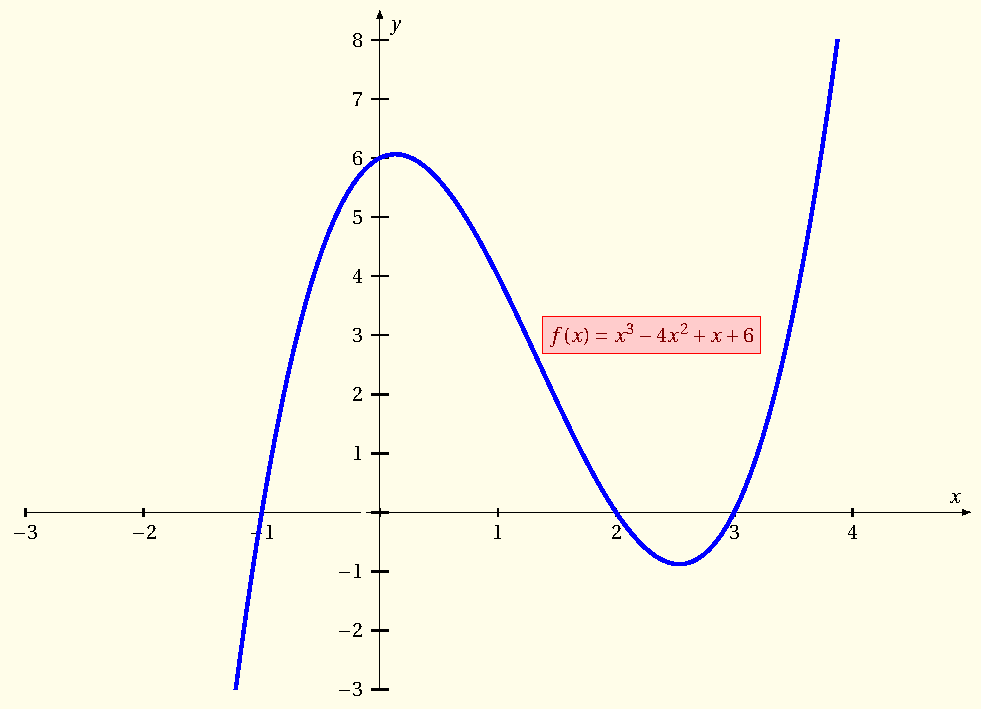
\includegraphics[scale=0.5]{17_home_antalcides_Calculo_pdf_image6-1.pdf}\caption{La función $f(x)=x^{3}-4x^{2}+x+6$}
\end{figure}

La imagen de esta función es $f(\R)=\R$. Esta función no tiene máximo
ni mínimo, no es creciente y tampoco es decreciente. No es inyectiva
y su función inversa no está definida.
\item Sea 
\begin{equation}
\funcreal{f}{[0,2]}\ \textrm{\ la función dada por\ }f(x)=x^{3}-4x^{2}+x+6\ \textrm{\ para todo\ }x\in[0,2]\label{func2}
\end{equation}
Observa que, aunque de forma deliberada uso la misma letra, $f$,
para representar la regla, la función definida en (\ref{func2}) es
muy diferente que la definida en (\ref{func1}). Aunque la regla es
la misma, en (\ref{func2}) solamente nos interesa lo que pasa en
el intervalo $[0,2]$. La imagen de esta función es $f([0,2])=[0,6]$.
Claramente, la función (\ref{func2}) es estrictamente decreciente,
tiene máximo y mínimo y es inyectiva. Su función inversa está definida
(aunque no sea fácil de calcular). 
\end{enumerate}

\section[Estudio descriptivo de las funciones elementales]{{Estudio descriptivo de las funciones elementales}}

En este curso se supone que ya tienes un conocimiento intuitivo de
las funciones elementales básicas (exponencial, logaritmo natural,
trigonométricas). En esta lección vamos a hacer un estudio descriptivo
de dichas funciones, es decir, no vamos a dar definiciones rigurosas
de las mismas y nos limitaremos a recordar sus propiedades más importantes.

\subsection{Funciones polinómicas y funciones racionales}

\noindent Las \emph{funciones polinómicas o polinomios} son las funciones
de la forma 
\[
P(x)=c_{0}+c_{1}x+c_{2}x^{2}+\cdots+c_{n}x^{n}
\]
donde $c_{0},c_{1},\dots,c_{n}$ son números reales llamados \emph{coeficientes}
del polinomio; $n\in\N$ es un número natural que, si $c_{n}\neq0$,
se llama grado del polinomio. Las funciones polinómicas tienen como
dominio natural de definición la totalidad de \R\ aunque con frecuencia
nos interesará estudiar una función polinómica en un intervalo.

Mientras que la suma, el producto y la composición de funciones polinómicas
es también una función polinómica, el cociente de funciones polinómica
da lugar a las llamadas \emph{funciones racionales}. Una función racional
es una función de la forma: 
\[
R(x)=\frac{P(x)}{Q(x)}
\]
donde $P$ (el numerador) y $Q$ (el denominador) son polinomios y
$Q$ no es el polinomio constante igual a $0$. La función $R$ tiene
como dominio natural de definición el conjunto\linebreak{}
$\{x\in\R:Q(x)\neq0\}$. Observa que las funciones polinómicas son
también funciones racionales (con denominador constante $1$).

Es inmediato que sumas, productos y cocientes de funciones racionales
son también funciones racionales; y la composición de dos funciones
racionales es también una función racional.

\subsection{Raíces de un número real}

Dados un número real $\,x\ge0\,$ y un número natural $\,k\geqslant2$,
hay un único número real \emph{mayor o igual que cero}, $z\ge0$,
que verifica que $\,z^{k}=x$. Dicho número real $\,z\,$ se llama
la \emph{raíz $k$-ésima o de orden $k$ de $x$} y se representa
por $\,\sqrt[k]{x}\,$ o por $\,x^{1/k}$. \begin{proposicion}{}{}
Sean $x,y\in\Rpo$, $k\in\N$. Se verifica que: 
\begin{enumerate}
\item $\ \sqrt[k]{x\,y}=\sqrt[k]{x}\,\sqrt[k]{y}$. 
\item La función $x\mapsto\sqrt[k]{x}$ es estrictamente creciente en $\Rpo$.
Es decir, se verifica que $x<y\,$ si, y sólo si, $\,\sqrt[k]{x}<\sqrt[k]{y}$. 
\end{enumerate}
\end{proposicion} Si $x<0$ y $k$ es \emph{impar} se define\footnote{Ver (\ref{notacionraices}) para el caso de raíces complejas.}
$\,\sqrt[k]{x}=-\sqrt[k]{|x|}$.
